\documentclass[12pt,italian]{report}
\usepackage{tesi}

%
%			INFORMAZIONI SULLA TESI
%			DA COMPILARE!
%

% CORSO DI LAUREA:
\def\myCDL{Corso di Laurea triennale in\\Informatica}

% TITOLO TESI:
\def\myTitle{ANALISI DEI DATI PER PROBLEMI DI\\ MEDICINA LEGALE}

% AUTORE:
\def\myName{Alessandro Beranti}
\def\myMat{Matr. Nr. 855489}

% RELATORE E CORRELATORE:
\def\myRefereeA{Prof. Dario Malchiodi}
\def\myRefereeB{Prof. Anna Maria Zanaboni}

% ANNO ACCADEMICO
\def\myYY{2018-2019}

% Il seguente comando introduce un elenco delle figure dopo l'indice (facoltativo)
%\figurespagetrue

% Il seguente comando introduce un elenco delle tabelle dopo l'indice (facoltativo)
%\tablespagetrue

%
%			PREAMBOLO
%			Inserire qui eventuali package da includere o definizioni di comandi personalizzati
%

% Package di formato
\usepackage[a4paper]{geometry}		% Formato del foglio
\usepackage[italian]{babel}			% Supporto per l'italiano
\usepackage[utf8]{inputenc}			% Supporto per UTF-8
%\usepackage[a-1b]{pdfx}			% File conforme allo standard PDF-A (obbligatorio per la consegna)

% Package per la grafica
\usepackage{graphicx}				% Funzioni avanzate per le immagini
\usepackage{hologo}					% Bibtex logo with \hologo{BibTeX}
%\usepackage{epsfig}				% Permette immagini in EPS
%\usepackage{xcolor}				% Gestione avanzata dei colori

% Package tipografici
\usepackage{amssymb,amsmath,amsthm} % Simboli matematici
\usepackage{listings}				% Scrittura di codice

% Package ipertesto
\usepackage{url}					% Visualizza e rendere interattii gli URL
\usepackage{hyperref}				% Rende interattivi i collegamenti interni

\usepackage{verbatim}

\setcounter{tocdepth}{4}
\setcounter{secnumdepth}{4}

\begin{document}

% Creazione automatica del frontespizio
\frontespizio
\beforepreface

% 
%			PAGINA DI DEDICA E/O CITAZIONE
%			facoltativa, questa è l'unica cosa che dovete formattare a mano, un po' come vi pare
%

{\raggedleft \large \sl Questo lavoro \`{e} dedicato a tutti gli studenti\\
	
	\vspace{2cm}
	
	``Io studio,\\ma studiate pure voi,\\che se studio solo io non serve a un c\dots o''
	
	\bigskip
	
	\--- Gli scarabocchi di Maicol \& Mirco\\
  
	\vspace{2cm}
	
	``No tale is so good \\ that it can't be spoiled \\ in the telling''
	
	\bigskip
	
	\--- Proverbio\\}
         
% 
%			PREFAZIONE (facoltativa)
%

%\prefacesection{Prefazione}
%Le prefazioni non sono molto comuni, tuttavia a volte capita che qualcuno voglia dire qualcosa che esuli dal lavoro in s\'e (come un meta-commento sull'elaborato), o voglia fornire informazioni riguardanti l'eventuale progetto entro cui la tesi si colloca (in questo caso \`e probabile che sia il relatore a scrivere questa parte).

%
%			RINGRAZIAMENTI (facoltativi)
%

\prefacesection{Ringraziamenti}
Questa sezione, facoltativa, contiene i ringraziamenti.

%
%			Creazione automatica dell'indice
%

\afterpreface

% 
%			CAPITOLO 1: Introduzione o Abstract
% 

\chapter{Introduzione}
\label{cap:introduzione}

Questo documento ha una duplice funzione: da un lato mostra un esempio completo di elaborato finale redatto in \LaTeX\ e conforme allo standard PDF/A, e dall'altro contiene suggerimenti e risposte a domande frequenti poste dagli studenti. Se ne raccomanda, pertanto, un'attenta lettura.

\chapter{Machine Learning}
Il termine Machine Learning, o apprendimento automatico in italiano, si riferisce alla capacità dei computer di apprendere e agire senza essere programmati esplicitamente.
Gli strumenti di machine learning si occupano di dotare i programmi della capacità di ``apprendere'' e adattarsi agli input forniti.
Al giorno d'oggi siamo circondati da tecnologie basate sull'apprendimento automatico:
\begin{itemize}
	\item software che rilevano lo spam a partire dai nostri messaggi e-mail, 
	\item motori di ricerca che imparano a ordinare i risultati di una query di ricerca al fine di mostrare prima quelli più rilevanti, 
	\item transazioni con carta di credito protette da un software che impara a rilevare le frodi, 
	\item fotocamere digitali che imparano a rilevare i volti, 
	\item assistenti digitali che imparano a riconoscere i comandi vocali, 
	\item veicoli autonomi addestrati a guidare senza intervento umano, 
	\item applicazioni scientifiche come la bioinformatica, la medicina e l'astronomia.
\end{itemize}
\section{Come funziona il Machine Learning}
\label{sec:Come funziona il Machine Learning}
Nel Machine Learning vengono usati metodi statistici che applicano un procedimento di induzione a partire da dati che rappresentano istanze di un problema, accoppiate con una possibile soluzione, per migliorare le prestazioni di algoritmi o fare previsioni più accurate.
La qualità e la dimensione dei dataset (collezione di dati), raccolti o resi disponibili e utilizzati nel processo sono fondamentali per il successo e l'accuratezza delle previsioni fatte.

Il processo parte da un domain set $X$, ovvero una raccolta arbitraria di dati, che rappresentano gli oggetti che si desidera etichettare. Essi possono essere già etichettati nel caso di apprendimento supervisionato come non esserlo nel caso non supervisionato. Questo set di dati rappresenta l'input dell'algoritmo di apprendimento che si è scelto di usare. Il risultato è un modello a cui è associato un errore di generalizzazione, ovvero la probabilità che non venga predetta l'etichetta corretta.
Il domain set può essere diviso in due sottoinsiemi: il \textit{training set}, insieme di dati che vengono scelti per compiere l'addestramento, e il \textit{test set} che viene utilizzato per valutare le prestazioni del modello predittivo.

Una categorizzazione dei compiti del machine learning si ha quando si considera l'output desiderato del sistema che può essere di diversi tipi:
\begin{itemize}
	\item classificazione, significa che il dato è categorico \cite{SupervisedMachineLearning} e viene fatta una divisione dei dati in classi o etichette. Può essere una classificazione binaria, nel quale le etichette sono soltanto due, oppure multiclasse, etichette sono tre o più,
	\item regressione, usata per predire un valore assimilabile a una quantità che varia in un insieme continuo, per esempio il prezzo di una casa date la dimensione e la metratura, \cite{SupervisedMachineLearning}
	\item clustering, in cui un insieme di input viene diviso in gruppi in modo che i singoli elementi siano simili agli altri punti dello stesso insieme e diversi dagli elementi degli altri; diversamente da quanto accade per la classificazione, i gruppi non sono noti prima, rendendolo tipicamente un compito non supervisionato. \cite{Introductiontodatamining}
\end{itemize}
Gli algoritmi di apprendimento automatico vengono tipicamente organizzati in quattro categorie, a seconda della natura del ``segnale'' utilizzato per l'apprendimento o del ``feedback'' disponibile al sistema di apprendimento. Queste categorie, anche dette paradigmi, sono:
\begin{itemize}
	\item Machine Learning supervisionato,
	\item Machine Learning non supervisionato,
	\item Machine Learning per rinforzo,
	\item Machine Learning semi-supervisionato.
	
\end{itemize}

\subsection{Apprendimento supervisionato}
Attraverso l’apprendimento supervisionato si cerca di costruire un modello partendo da dati di addestramento etichettati, a partire dai quali si tenta di fare previsioni su dati non disponibili o futuri. Con il termine ``supervisione'' si intende quindi che nell'insieme dei campioni (o dataset), i segnali di output desiderati sono già noti poiché precedentemente etichettati.
Nell'apprendimento supervisionato l'output può essere sia numerico che categorico, quindi può trattarsi rispettivamente di regressione e classificazione; siccome il tirocinio ha riguardato solo quest'ultima d'ora in avanti parleremo di classificazione.

Esistono molti algoritmi per svolgere apprendimento supervisionato, durante il tirocinio ho avuto modo di usare:
\begin{itemize}
	\item Support Vector Machine,
	\item Decison Tree Classifier,
	\item Random Forest Classifier,
	\item Gaussian Naive Bayes,
	\item Linear Discriminant Analysis,
	\item Multi-Layer Perceptron Classifier.
\end{itemize}

\subsubsection{Support Vector Machine}
\label{sec:SVC}
Il Support Vector Machine (SVM) è un algoritmo di apprendimento automatico supervisionato che può essere usato sia per scopi di classificazione che di regressione, si può applicare sia a problemi binari, sia a problemi multiclasse. Nel paragrafo seguente verrà descritto solo la versione per la classificazione binaria poichè è quella che ho usato durante il tirocinio.

L'SVM è basato sull'idea di riuscire a trovare un iperpiano che divida al meglio un set di elementi in due classi distinte \cite{LectureNotesNg}. Definiamo alcuni elementi che ci serviranno successivamente.


\begin{itemize}
	\item Iperpiano: nel caso in cui si abbiano solo due dimensioni spaziali nel qualche si trovano le descrizioni degli oggetti da classificare $x_1$ e $x_2$, l'iperpiano è raffigurato come una linea che separa un insieme di dati \cite{LectureNotesNg}. Nel caso in cui le dimensioni siano 3, l'iperpiano è raffigurato come un piano, ( cfr. Figura 1).
	%\begin{figure}[h]
	%	\centering
	%	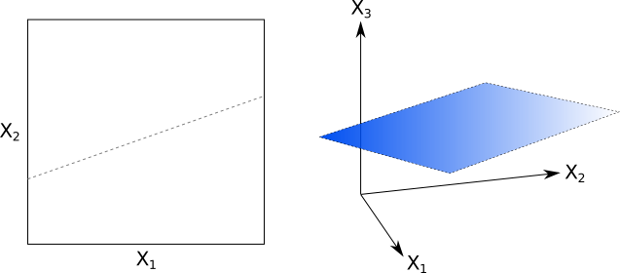
\includegraphics[width = 50mm]{immagini/Iperpiano-3-dimensioni}
	%	\caption{A sinistra grafico bidimensionale e destra tridimensionale}
	%\end{figure}
	Con più di 3 dimensioni viene definito ``iperpiano''.
	\item Support Vector: chiamati vettori di supporto in italiano, sono i punti che si trovano piu vicini all'iperpiano che divide i dati.
	\item Margine: è la distanza tra i vettori di supporto di due classi diverse. A metà di questa distanza viene tracciato l'iperpiano, (cfr. Figura 2).
\end{itemize}

\begin{figure}[h]
	\centering
	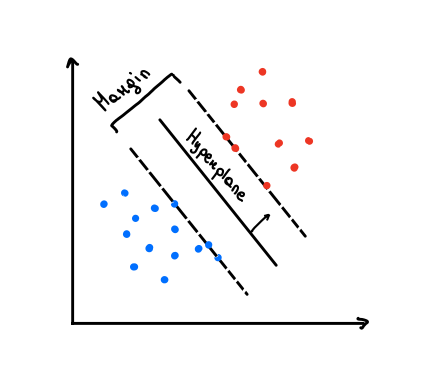
\includegraphics[width = 47mm]{immagini/marginEhiperplane}
	\caption{Iperpiano e margine}
\end{figure}

Il Support Vector Machine ha l'obiettivo di identificare l'iperpiano che divide meglio i vettori di supporto in classi. Esistono due algoritmi diversi a seconda se esista o meno l'iperpiano.

\begin{itemize}
	\item Nel caso in cui esista e in particolare ce ne sia più di uno cerca quello con il margine più alto tra i vettori di supporto in modo da evidenziare meglio la divisione tra i dati. La massimizzazione del margine porta ad avere degli iperpiani che tendono a minimizzare le probabilità di errore quando classificano nuovi dati. 
	\item Se l'iperpiano cercato non esiste, Support Vector Machine usa una mappatura non lineare per trasformare i dati di training $X$, in uno spazio di dimensione superiore rispetto a quello dei dati originali in modo che le immagini dei dati di due classi siano separati da un iperpiano, che sarà scelto per la suddivisione dei dati. 
\end{itemize}

In dati linearmente separabili è possibile individuare un iperpiano in cui si possono distinguere due semispazi. Nella figura 3 è visibile come sia possibile disegnare un numero infinito di linee rette per separare i diversi elementi. Il problema è trovare quale tra le infinite rette risulti ottimale, ossia quella che, a fronte di una generica nuova osservazione, classifichi nel modo corretto l'osservazione.

\begin{figure}[h]
	\centering
	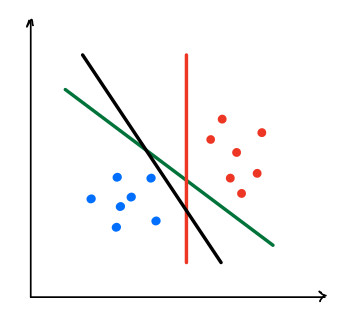
\includegraphics[width = 60mm]{immagini/linearmente-separabili}
	\caption{Infinite rette possono separare gli elementi}
\end{figure}

Dato un training set etichettato:

\begin{center}
	\[
	\ (x_1, y_1), ..., (x_n, y_n)
	\ \forall i 
	\ x_i \in R^{d},
	\ y_i \in  \{ -1, +1 \}
	\]
\end{center}
dove $x_i$ sono i punti da classificare e $y_i$ sono le etichette.

Un iperpiano è definito come 
\begin{center}
	\[w_0 + w_1z_1 + w_2z_2 +...+ w_mz_m= 0,\]
\end{center}
dove $\omega$ è il vettore di peso, $z$ è il vettore di caratteristiche di input e $w_0$ è il bias.
In sostanza in $m$ dimensioni un iperpiano di separazione è una combinazione lineare di tutte le dimensioni uguagliate a 0.
Ragionando a due dimensioni per semplificare il problema abbiamo che 
\begin{center}
	\[w_0 + w_1z_1 + w_2z_2 = 0.\]
\end{center}
I punti che stanno sopra l'iperpiano e che rappresentano un classe soddisfano la seguente condizione:
\begin{center}
	\[w_0 + w_1z_1+w_2z_2 > 0,\]
\end{center}
mentre qualsiasi punto che si trova sotto l'iperpiano, appartiene all'altra classe, che è soddisfatta dalla seguente condizione :
\begin{center}
	\[w_0 + w_1z_1+w_2z_2 < 0,\]
\end{center}
L'algoritmo di apprendimento per SVM, in realtà, riscrive queste condizioni in modo più stringente:
\begin{center}
	\[w_0 + w_1z_1+w_2z_2 \geq 1,
	\ if
	\ y=1,\]
	\[
	\ w_0 + w_1z_1+w_2z_2 \leq 1 
	\ if
	\ y = -1,
	\]
	\[ y \in (-1, +1)\]
\end{center}
Se il vettore dei pesi è indicato da $w$ e $\parallel w \parallel$ è la sua norma, allora la dimensione del margine massimo è 
\begin{center}
	\[ \frac{1}{\left || w \right ||} + \frac{1}{\left || w \right ||} = \frac{2}{\left || w \right ||},\]
\end{center}
ciò significa che minimizzando la norma del vettore peso $w$, avremo margine massimo che determina l'iperpiano ottimale.

Non è però sempre possibile dividere i dati tramite un iperpiano, come esemplificato in Figura 4.

\begin{figure}[h]
	\centering
	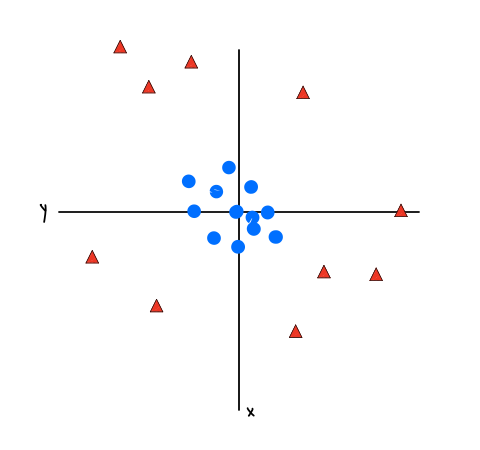
\includegraphics[width = 70mm]{immagini/nonLineare}
	\caption{Non sempre è possibile dividere i dati linearmente}
\end{figure}

Per utilizzare la classificazione tramite iperpiani anche per dati che avrebbero bisogno di funzioni non lineari per essere separati, è necessario ricorrere alla tecnica degli spazi immagine ($feature$ $spaces$). Questo metodo, che sta alla base della teoria delle SVM, consiste nel mappare i dati iniziali in uno spazio di dimensione superiore.  Presupponendo quindi $m > n$, per la mappa si utilizza una funzione
\begin{equation}
	\phi: \mathbb{R}^{n} \rightarrow \mathbb{R}^{m},
\end{equation}
attraverso la funzione $\phi$ i dati vengono mappati in uno spazio a più dimensioni, ciò comporta che i dati potrebbero essere linearmente separabili e quindi sarebbe possibile trovare un iperpiano che li separi. \cite{LectureNotesNg}

La tecnica degli spazi immagine è particolarmente interessante per algoritmi che utilizzano i dati di training $x_i$ solo attraverso prodotti scalari $x_i \cdot x_j$. In questo caso nello spazio $\mathbb{R}^{m}$ non si devono trovare esplicitamente $\phi(x_i)$ e $\phi (x_j)$ ma basta calcolare il loro prodotto scalare $\phi (x_i) \cdot \phi (x_j)$. Per rendere semplice questo ultimo calcolo, che in spazi di dimensioni elevate diventa molto complicato, si utilizza una funzione detta \textit{kernel} che restituisce direttamente il prodotto scalare delle immagini:
\begin{equation}
K(x_i, x_j) = \phi (x_i) \cdot \phi (x_j),
\end{equation}
Esistono svariati \textit{kernel}, i più utilizzati sono:
\begin{itemize}
	\item il kernel lineare: $K(x, y) = x \cdot y$,
	\item il kernel polinomiale: $K(x, y) = (x \cdot y)^{d}$ oppure $K(x, y) = (1 + x \cdot y)^{d}$,
	\item il kernel gaussiano: $K(x,y) = \exp (- \left || x-y \right || ^2)/(2 \sigma 2)$,
	\item il kernel sigmoide: $K(x,y) = \tanh(k x \cdot y - \delta)$.
\end{itemize}

\subsubsection{Decision Tree Classifier}
Il Decision Tree Classifier è un metodo di apprendimento supervisionato usato sia per scopi di classificazione che di regressione. Utilizza un albero decisionale, \textit{decision tree}, composto da \cite{DataMiningandKnowledgeDiscoveryHandbook}:
\begin{itemize}
	\item nodi non terminali: rappresentano un test su uno o più caratteristiche,
	\item ramo: rappresenta un esito del test,
	\item foglia: rappresenta una possibile classe.
\end{itemize}

Dato un insieme di dati è possibile costruire un numero esponenziale di alberi di decisione. Alcuni alberi sono più efficienti di altri ma trovare l'albero ottimo è una cosa computazionalmente infattibile a causa dello spazio esponenziale nel quale bisogna cercare. Tuttavia esistono algoritmi che riescono, in un tempo ragionevole, a trovare un albero efficiente anche se non corrisponde all'ottimo. Questi algoritmi spesso implementano una strategia greedy che crea l'albero facendo una serie di decisioni localmente ottime su quale caratteristica dei dati usare per partizionare i dati. \cite{Introductiontodatamining}
Uno di questi algoritmi è l'algoritmo di Hunt nel quale l'albero di decisione viene costruito ricorsivamente partizionando il training set in sottoinsiemi sempre più piccoli. Sia $D_t$ l'insieme dei dati di training che sono associati al nodo $t$ e sia $y = {y_1, y_2,...,y_c}$ le etichette. La definizione ricorsiva dell'algoritmo di Hunt è la seguente. \cite{Introductiontodatamining}
\begin{itemize}
	\item se tutti i dati in $D_t$ appartengono alla stessa classe $y_t$, allora $t$ è una foglia etichettata come $y_t$
	\item se $D_t$ contiene dati che appartengono a più di una classe, viene selezionata una caratteristica per eseguire un test per partizionare i dati in sottoinsiemi più piccoli. Viene creato un nodo figlio per ogni risultato della condizione del test e i dati in $D_t$ vengono divisi in base al risultato del test. L'algoritmo viene applicato in modo ricorsivo ad ogni nodo figlio.
\end{itemize}

La misura di selezione degli attributi è un'euristica per selezionare il criterio di suddivisione che divide i dati in modo da massimizzare l'omogeneità dei sottoinsiemi di dati. I più famosi sono l'entropia e l'indice di Gini. \cite{DataMiningandKnowledgeDiscoveryHandbook}

\subsubsection{Random Forest Classifier}
Il Random Forest Classifier è un algoritmo di apprendimento supervisionato. Esso considera più alberi di decisione che operano come un insieme. Ogni albero della foresta genera una previsione e quella che compare più frequentemente diventa la previsione del modello. \cite{RandomForest}

Il concetto fondamentale dietro una foresta casuale risiede nel fatto che un grande numero di alberi non correlati tra loro che operano insieme tendono a essere più efficienti di un singolo albero.

La bassa correlazione è la chiave, modelli non correlati possono produrre previsioni d'insieme più accurate di qualsiasi singola previsione. La ragione risiede nel fatto che, anche se alcuni alberi potrebbero sbagliare, molti altri avranno ottenuto la previsione corretta.
\subsubsection{Gaussian Naive Bayes}
Il Gaussian Naive Bayes è uno dei più semplici algoritmi di apprendimento supervisionato, e si basa sul teorema di Bayes. L'algoritmo assume che l'effetto di una particolare caratteristica in una classe sia indipendente dalle altre caratteristiche. Anche se le caratteristiche sono interdipendenti, esse vengono comunque considerate in modo indipendente\cite{Mitchell97}. Questa ipotesi, a cui ci si riferisce come indipendenza condizionale di classe, semplifica il calcolo.
Applicando il teorema di Bayes si ha
\begin{equation}
P(y | X) = \frac{P(X | y) P(y)}{P(X)},
\end{equation}
dove $y$ è un'etichetta e $X = (z_1, z_2, z_3,...,z_n)$ è il corrispondente vettore di caratteristiche.

Siccome abbiamo assunto che le caratteristiche siano indipendenti possiamo dire che:
\begin{equation}
P(y| z_1,..., z_n) = \frac{P(z_1|y) P(z_2|y)...P(z_n|y)P(y)}{P(z_1)P(z_2)...P(z_n)}.
\end{equation}
Poiché il denominatore rimane costante per un determinato input possiamo rimuoverlo e scrivere:
\begin{equation}
P(y| z_1,..., z_n) \propto P(y) \prod_{i=1}^{n} P(z_i|y).
\end{equation}
Ora dobbiamo creare un modello per classificare. Lo facciamo trovando la probabilità di un dato insieme di input per tutti i possibili valori di $y$ e prendendo l'output con la massima probabilità:
\begin{equation}
y = \arg\max P(y) \prod_{i=1}^{n} P(z_i|y).
\end{equation}
Rimane solo da calcolare $P(y)$ e $P(z_i|y)$, che sono ricavabili dal dataset dato in input al sistema.

Nel Gaussian Naive Bayes si presume che i valori continui associati a ciascuna caratteristica siano distribuiti secondo un modello gaussiano. 

Sulla base di questa assunzione è quindi possibile scrivere le probabilità condizionate che compaiono in (6) nel modo seguente
\begin{equation}
P(z_i|y) = \frac{1}{\sqrt{2\pi \sigma_y^2}} e^{-\frac{(z_i-\mu_y)^2}{2\sigma_y^2}},
\end{equation}
dove $\mu_y$ è la media e $\sigma_y$ la deviazione standard.
\subsubsection{Linear Discriminat Analysis}
Il Linear Discriminat Analysis è un algoritmo di apprendimento supervisionato il cui scopo è quello di trovare una combinazione lineare di caratteristiche che caratterizza o separa due o più classi di oggetti. La combinazione risultante può essere utilizzata come classificatore o anche per la riduzione della dimensionalità. \ref{sec:riduzione}

Il processo prevede di proiettare i dati in input su un sottospazio lineare dalle direzioni che massimizzano la divisione tra le classi. La dimensione dell'output è necessariamente inferiore al numero di classi, quindi questa è, in generale, una riduzione della dimensionalità piuttosto forte, e ha senso solo in un ambiente multiclasse.

%Linear Discriminant Analysis può essere derivato utilizzando la regola di Bayes
%\begin{equation}
%P(y=k|X) = \frac{P(X|y=k) P(y=k)}{P(X)} = \frac{P(X|y=k) P(y=k)}{\sum_{l}P(X|y=l) \cdot P(y=l)}
%\end{equation}
%e selezionamo la classe $k$ che massimizza questa probabilità condizionata.
\subsubsection{Reti Neurali Multi-Strato}
Le reti neurali multi-strato sono un modello che utilizza l'algoritmo ``backpropagation'', basato sulla minimizzazione dell'errore, per compiere apprendimento supervisionato. L'idea di base è quella del neurone umano e della rete di neuroni che compone il nostro cervello. Il componente principale di una rete neurale è detto neurone o percettrone. Esso è identificato da $n$ pesi reali $w_1, w_2,...,w_n$ e quando riceve una serie di input $x_1,x_2,...,x_n$ li moltiplica per i pesi corrispondenti, viene così prodotto un valore $v$ sommando i prodotti ottenuti a cui viene sommato un termine di bias. \cite{multilayerPerceptron}  L'output della rete è ottenuto calcolando una particolare funzione, detta funzione di attivazione, usando $v$ come argomento.

\begin{figure}[h]
	\centering
	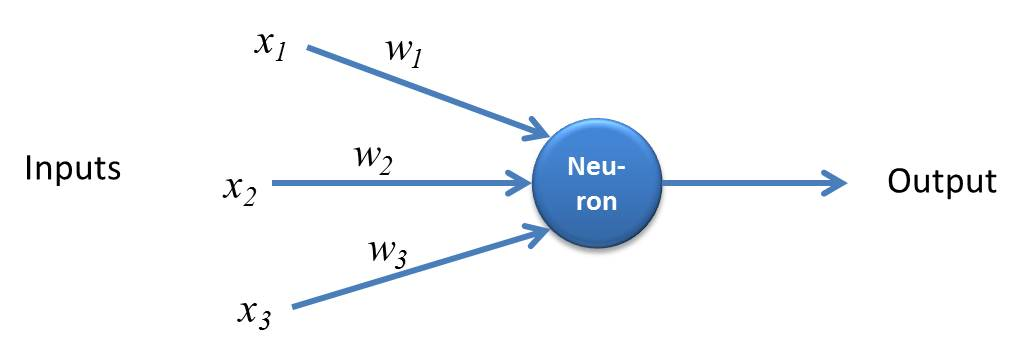
\includegraphics[width = 90mm]{immagini/Perceptron}
	\caption{Visualizzazione di un percettrone}
\end{figure}


Una rete con un solo percettrone è chiamata a singolo livello. Esistono poi le reti multistrato, sono reti i cui percettroni sono disposti su più livelli, come indicato in Fgigura 8. Esistono tre tipi di livelli: 
\begin{itemize}
	\item livello input: costituito da un insieme di neuroni che rappresentano le caratteristiche in input,
	\item livello output: riceve i valori dall'ultimo livello hidden presente e li trasforma in valori di output, 
	\item livello hidden: livelli intermedi tra input e output, 
\end{itemize}


In questa rete ogni nodo, esclusi quelli di input, usa una funzione di attivazione non lineare per modellare il comportamento.

\begin{figure}[h]
	\centering
	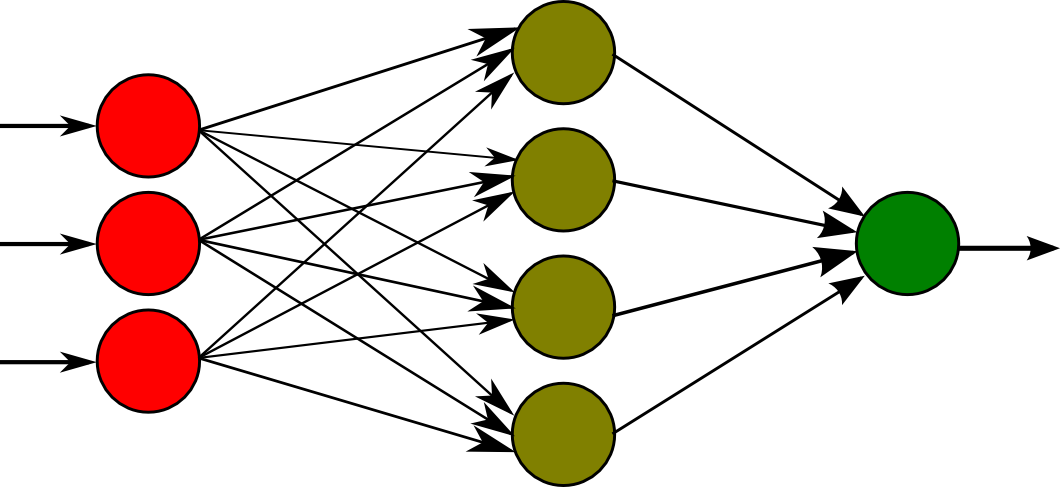
\includegraphics[width = 80mm]{immagini/Multilayer-Perceptron}
	\caption{Visualizzazione di una rete multistrato; in rosso il livello di input, al centro il livello hidden, in verde a destra il livello di output}
\end{figure}
Esistono diverse funzioni di attivazione:
\begin{itemize}
	\item Identity: $f(x) = x$,
	\item Logistic: $f(x) = \frac{1}{1 + e^{-x}}$,
	\item Tanh: $f(x) = \tanh(x)$,
	\item Relu: $f(x) = \max(0, x)$.
\end{itemize}
L'output $y$ viene calcolato nel seguente modo: 
\begin{equation}
y = \Phi \left ( \sum_{i=1}^{n}w_ix_i + b \right ) = \Phi (w^{T}x + b),
\end{equation}
dove $w$ è il vettore di pesi, $x$ è il vettore di input, $b$ è il bias e $\Phi$ è la funzione di attivazione.

Il processo di addestramento del Multi-Layer Perceptron avviene mediante una continua regolazione dei pesi delle connessioni dopo l'elaborazione di ogni oggetti nel dataset a disposizione. Questa regolazione si basa sull'errore nell'output ed dà vita ad un processo di apprendimento chiamato ``backpropagation''. Tale processo continua fino a che non si verifica un criterio di fine apprendimento (per esempio, dopo un numero finito di iterazioni, o quando l'errore non scende sotto una soglia prefissata).
Il processo continua fino a quando l'errore non raggiunge il valore più basso. \cite{multilayerPerceptron}
\subsection{Apprendimento non supervisionato}
Nell’apprendimento non supervisionato, al contrario di quello supervisionato abbiamo dei dati senza etichetta. Le tecniche di apprendimento non supervisionato mirano a estrarre, in modo automatico, della conoscenza a partire da basi di dati, e questo avviene senza una specifica conoscenza dei contenuti da analizzare. Un esempio tipico di questi algoritmi lo si ha nei motori di ricerca. Questi programmi, data una o più parole chiave, sono in grado di creare una lista di link rimandanti alle pagine che l'algoritmo di ricerca ritiene attinenti alla ricerca effettuata. \cite{unsupervisedlearning}
I principali algoritmi utilizzati in ambito non supervisionato fanno riferimento a tecniche di clustering e a regole di associazione.
\subsection{Apprendimento per rinforzo}
Il terzo tipo di apprendimento automatico è l’apprendimento per rinforzo. L’obiettivo di questo tipo di apprendimento è quello di costruire un sistema che attraverso le interazioni con l’ambiente migliori le proprie performance. \cite{unsupervisedlearning}

Per poter migliorare le funzionalità del sistema vengono introdotti dei rinforzi, ovvero segnali di ricompensa. Questo rinforzo non è dato dalle etichette, ma è una misurazione sulla qualità delle azioni intraprese dal sistema. Per questo motivo non può essere assimilato all'apprendimento supervisionato.
Potremmo trovare questo tipo di apprendimento ad esempio nell’addestramento di un sistema per il gioco degli scacchi.

Inizialmente le mosse saranno del tutto casuali e senza una logica. Dal momento in cui il sistema riceverà dei feedback positivi, come ad esempio nel caso in cui mangi una pedina avversaria, allora riceverà un peso maggiore e conseguentemente un rinforzo positivo su quell’azione. Contrariamente in caso di azione negativa, il valore dei pesi su quell’azione andrà in decremento.

Conseguentemente a questi rinforzi, il sistema darà maggior peso alle mosse che gli hanno portato maggiori benefici e tenderà a replicare lo stesso comportamento su nuove mosse future.
\subsection{Apprendimento semi supervisionato}
Può essere visto come un quarto tipo di apprendimento automatico. In questo caso, al contrario dell’apprendimento non supervisionato, abbiamo che di tutti i dati presenti nel training set, solo pochi di essi sono stati etichettati.\cite{semisupervised}

%			CAPITOLO 2


\chapter{Dataset}
Un dataset è una collezione di dati, comunemente corrisponde al contenuto di una singola tabella nella quale una colonna corrisponde a una caratteristica e ogni riga ad una singola osservazione o istanza. Gli algoritmi di Machine Learning utilizzano i dataset per "apprendere". Quanto più un dataset è ricco di osservazioni tanto più l'algoritmo che lo utilizza sarà in grado di fornire prestazioni e accuratezza in output. 

\section{Iris}
Durante il tirocinio, inizialmente, per prendere familiarità con gli strumenti e algoritmi necessari a compiere lo studio, ho utilizzato il dataset Iris. Esso è un dataset multivariato introdotto da Ronald Fisher nel 1936. Consiste in 150 istanze di fiori iris e classificate secondo tre specie: Setosa, Virginica e Versicolor.
Le variabili considerate sono lunghezza e larghezza di sepalo e petalo.
\begin{figure}[h]
	\centering
	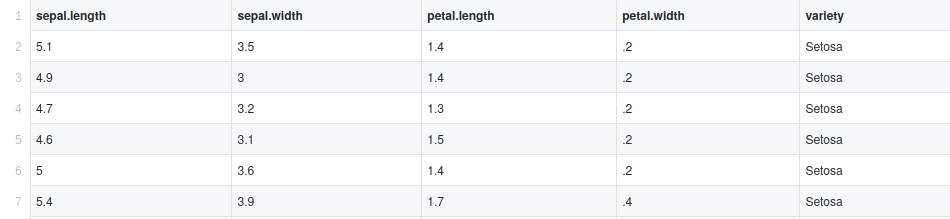
\includegraphics[width = 150mm]{immagini/Iris}
	\caption{Visualizzazione di un estratto del dataset Iris}
\end{figure}
\section{Incidenti Stradali}
Apprese le basi del Machine Learning ho iniziato a lavorare con il dataset ``Incidenti Stradali'', questo dataset è stato fornito da medici legali e raccoglie, tristemente, i decessi causati appunto da incidenti stradali. Sono state raccolte 131 istanze e ognuna rappresenta una persona deceduta. Il dataset è organizzato in vari livelli di dettaglio. Un primo livello è composto dalle  caratteristiche basilari:
\begin{itemize}
	\item numero del verbale, verrà usato come indice univoco,
	\item data del decesso,
	\item sesso,
	\item anni,
	\item peso,
	\item altezza,
	\item BMI, indice di massa corporea.
\end{itemize}
Successivamente sono raccolte tutte le ossa rotte durante l'incidente con etichette che vanno da 0, nessuna lesione, a 4, lesione massima.
Successivamente sono descritti i totali delle rotture avvenute nei distretti di:
\begin{itemize}
	\item testa,
	\item torace,
	\item addome,
	\item scheletro,
\end{itemize}
Ogni distretto è poi diviso più nello specifico in singole ossa. (cfr. Figura 9)
\begin{figure}[h])
	\centering
	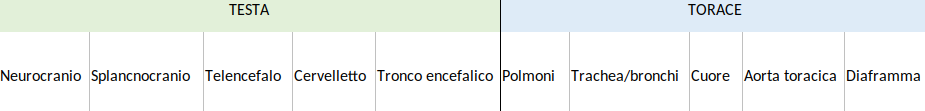
\includegraphics[width = 160mm]{immagini/testa-torace-dataset}
	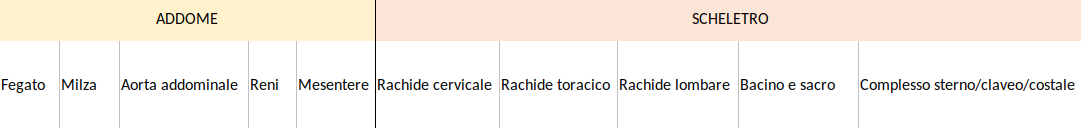
\includegraphics[width = 160mm]{immagini/addome-scheletro-dataset}
	\caption{Suddivisione caratteristiche dettagliate}
\end{figure}

Il dataset ha inoltre due ulteriori livelli di dettaglio. Esso contiene infatti anche dati più specifici riguardanti la frattura o meno di singole ossa raggruppate in:
\begin{itemize}
	\item cranio,
	\item rachide,
	\item torace - gabbia toracica,
	\item bacino,
	\item arti superiori,
	\item arti inferiori.
\end{itemize}
In ultimo è registrato il mezzo che ha investito la persona. Questo è il label set, la y dei modelli descritti al capitolo precedente. Tutti gli esperimenti effettuati in fase di studio sono incentrati sul cercare di classificare il tipo di mezzo, leggero ovvero auto, etichettato con 0, o pesante, con etichetta 1, che ha investito l'individuo.

Nel mio studio mi sono limitato a considerare le caratteristiche basilari, i totali e quelle riportate in Figura 7.
\section{Riduzione della Dimensionalità}
\label{sec:riduzione}
Nei problemi di classificazione di Machine Learning ci sono spesso molte caratteristiche da tenere in considerazione, basti pensare che il dataset ``Incidenti Stradali'' al completo ha circa 350 caratteristiche. Per dataset con molte dimensioni la riduzione della dimensionalità è un pratica importante svolta prima di applicare algoritmi di Machine Learning per evitare l'effetto chiamato \textit{curse of dimensionality}, ``maledizione della dimensionalità''. Il problema sorge nel momento in cui la dimensionalità aumenta e lo spazio aumenta così rapidamente che i dati disponibili diventano radi, sparsi. In ambito statistico questa scarsità è problematica in quanto i dati necessari a supportare il risultato aumentano in modo esponenziale.
Inoltre dati con molte dimensioni possono causare problemi di \textit{overfitting}, ovvero il sistema in qualche modo impara e memorizza il risultato, si adatta (\textit{fitting}) troppo bene (\textit{over}) ai dati di training perdendo di generalità. Il modello sembra perfetto per i dati di training ma quando si prova ad applicarlo ai dati di test si verificano molti errori.
Per questo motivo viene effettuata una riduzione della dimensionalità in modo da eliminare le caratteristiche più irrilevanti e lasciare spazio a quelle rilevanti. 

In questo contesto entrano in gioco algoritmi di riduzione della dimensionalità come PCA e t-SNE.

\subsection{PCA}
L'idea alla base del pricipal component analysis (PCA), o analisi delle componenti principale, è di ridurre la dimensione di un dataset che contiene un grande numero di caratteristiche correlate, mantenendo il più possibile la varianza presente nel dataset. Quello che si fa è selezionare le componenti principali, che non sono correlate tra di loro e che sono ordinate in modo tale che le prime  mantengano la maggior parte di varianza presente in tutte le caratteristiche iniziali. \cite{pca}

L'idea è di trattare le caratteristiche come una matrice $M$ e trovare gli autovettori per $M M^{T}$ o $M^{T}M$. 

La matrice di questi autovettori può essere vista come una rotazione nello spazio. 
\begin{figure}[h]
\centering
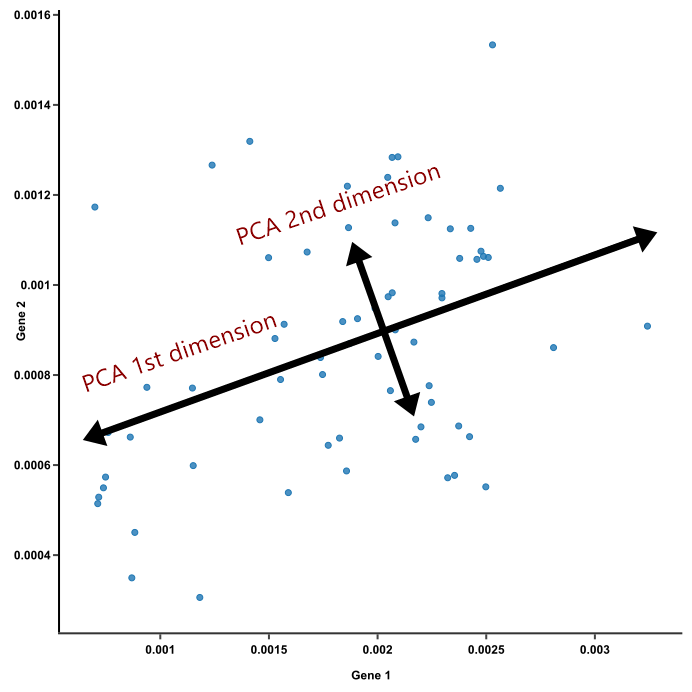
\includegraphics[width = 100mm]{immagini/pca}
\caption{Dimensioni trovate tramite PCA \cite{pcaFigura}}
\end{figure}


Quando si applica questa trasformazione dei dati, l'asse corrispondente all'autovettore principale è quello nel quale i dati sono più sparsi, ovvero l'asse nel quale la varianza dei dati è massimizzata.

Detto in altro modo, i punti possono essere osservati meglio se distesi lungo questo asse, con piccole deviazioni da esso. Allo stesso modo, l'asse corrispondente al secondo autovettore (l'autovettore corrispondente al secondo autovalore più grande) è l'asse lungo il quale la varianza delle distanze dal primo asse è maggiore, e così via fino al numero di dimensioni che si è scelto di tenere.

Ma come funziona esattamente? 
Per prima cosa si costruisce la matrice dei dati A nel quale ogni colonna corrisponde ad una caratteristica e ogni riga ad una istanza. Successivamente si calcola la media di ogni colonna e la si sottrae ad ogni elemento della matrice, ottenendo così la matrice B.

A questo punto viene calcolata la matrice di covarianza. Ogni valore di covarianza assume un segno: se positivo significa che c'è una correlazione positiva, al contrario, se negativa, c'è una correlazione inversa.

La matrice appena calcolata serve per poter calcolare gli autovalori, operatori che si basano sul fatto che moltiplicando o dividendo un vettore cambia solo la sua lunghezza e non la direzione. Un autovalore $\lambda$ è tale se risolve $Av = \lambda v$, con $A$ matrice quadrata e $v$ vettore che viene definito autovettore. 

Esempio: A=$\left [\begin{matrix}
1&1\\8&1
\end{matrix}\right]
$ 
e
$v=\left[\begin{matrix}
1\\2
\end{matrix} \right]$, allora 5 rappresenta un autovalore in quanto verifica l'equazione

Per calcolare gli autovalori di una matrice è possibile risolvere la seguente equazione
\begin{equation}
det(A - \lambda I) = 0,
\end{equation}
dove $I$ è la matrice identità e $det$ rappresenta il determinante della matrice.

Allo stesso modo è possibile calcolare gli autovettori corrispondenti agli autovalori calcolati precedentemente risolvendo l'espressione e trovando $v$:
\begin{equation}
det(A - \lambda I) v = 0.
\end{equation}
Gli autovettori trovati formeranno gli assi del nuovo sistema di riferimento di dimensioni più piccole rispetto a quello iniziale. Tuttavia gli autovettori definiscono solo le dimensioni dell'asse poiché hanno tutti lunghezza 1, di conseguenza per decidere quale autovettore vogliamo eliminare per il nostro sottospazio di dimensione inferiore dobbiamo vedere gli autovalori degli autovettori. Quello che faremo sarà eliminare gli autovettori con autovalori più bassi in quanto hanno il minor numero di informazioni sulla distribuzione dei dati al loro interno. Quello che viene fatto è ordinare gli autovalori dal più grande al più piccolo e prendere i primi $k$ autovettori corrispondenti.

In ultimo dobbiamo formare le componenti principali, per farlo calcoliamo:
\begin{equation}
CP = W^{T} \cdot B^{T}
\end{equation}
dove $CP$ è la matrice costituita dalle componenti principali, $W^{T}$ è la matrice formata usando gli autovettori che abbiamo scelto di mantenere precedentemente di cui prendiamo la trasposta, $B^{T}$ è la trasposta della matrice B precedentemente calcolata.
Quello che si ottiene sono i dati originali ma inseriti nello spazio considerando come assi di riferimento gli autovettori calcolati.

Sebbene PCA sia uno degli algoritmi più famosi e usati poiché è veloce, facile da usare e intuitivo ha un problema: è una tecnica lineare, questo significa che non è in grado di trovare delle dipendenze non lineari che gli consentono di tornare ad uno stato precedente. 

t-SNE non è limitato da proiezioni lineari il che significa che può adattarsi ad ogni tipo di dataset.
\subsection{t-SNE}
t-SNE, o t-Distributed Stochastic Neighbor Embedding, è una tecnica di riduzione della dimensionalità non lineare. Utilizza una struttura locale nel quale punti aventi molte dimensioni vengono mappati nello spazio usando un numero inferiore di dimensioni in modo che le distanze tra i punti rimangano quasi le stesse.
 
L'algoritmo prevede tre step.
\begin{itemize}
	\item Misura le somiglianze tra i punti nello spazio a molte dimensioni e, per ogni punto $x_i$, centra una distribuzione gaussiana sopra di esso. Viene misurata la densità di tutti gli altri punti $x_j$ sotto questa distribuzione.
	Successivamente viene normalizzata la curva per tutti gli altri punti.
	Questo ci dà un set di probabilità ($Pij$) che sono proporzionali alle somiglianze, ciò significa che se i punti $x_1$ e $x_2$ hanno valori uguali sotto questa distribuzione gaussiana, le loro proporzioni e somiglianze sono uguali. La distribuzione può essere manipolata usando quella che viene chiamata perplessità, la quale influenza la varianza della distribuzione, ovvero quanto è ampia la curva, che a sua volta influenza  il numero dei vicini di ogni punto. Il normale range della perplessità è tra 5 e 50.
	\item Simile al primo ma anziché usare una distribuzione gaussiana usa Student. Essa ci fornisce un secondo set di probabilità $Q_ij$ in uno spazio ridotto. La t-distribution ha code più lunghe rispetto alla gaussiana, questo fornisce una migliore visualizzazione della distanza dei punti. (cfr. Figura 9)
	
	\begin{figure}[h]
		\centering
		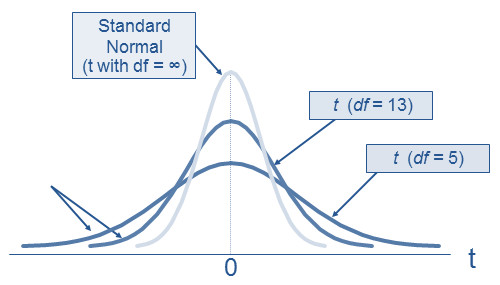
\includegraphics[width = 79mm]{immagini/t-dist1}
		\caption{In verde distribuzione gaussiana vs t-Student in blu. La forma della distribuzione t-student è data dai gradi di libertà che si riferiscono al numero di osservazioni indipendenti all'interno dei dati}
	\end{figure}
	\item Vogliamo ora che le probabilità $Q_{ij}$ calcolate nello spazio ridotto riflettano al meglio possibile le $P_{ij}$ calcolate usando lo spazio con più dimensioni. 
	Misuriamo la differenza tra le distribuzioni di probabilità degli spazi delle due dimensioni usando la divergenza di Kullback-Liebler (KL) che confronta efficacemente valori di $P_{ij}$ e $Q_{ij}$ di grandi dimensioni. Infine, usiamo la tecnica della discesa gradiente per ridurre al minimo la funzione di costo KL. \cite{t-SNE}
\end{itemize}

Nel capitolo 3 vedremo concretamente come utilizzare PCA e t-SNE per ridurre la dimensione del dataset Incidenti Stradali.



% 
%			CAPITOLO 3: Esperimenti
% 

\chapter{Esperimenti}
\label{cap3}
Durante il tirocinio ho effettuato diversi esperimenti a partire dal dataset fornito prendendo in considerazione 

\section{Model Selection}

\subsection{Scelta degli Iperparametri}

\begin{equation}
x_i(n) = a_{i1}u_1(n) + a_{i2}u_2(n) + \cdots + a_{iJ}u_J(n) \, .
\label{eq:multimix}
\end{equation}

\subsection{Scalare i dati}


\section{Errore di Generalizzazione}
\label{sec:errore}


\subsection{Training}



\subsection{Cross Validation}



\section{Risultati Ottenuti}
\label{sec:risultati}


% 
%			CAPITOLO 4: Conclusioni e sviluppi futuri
% 
\chapter{Conclusioni}

Nelle conclusioni si tirano le somme di quanto realizzato, facendo un riassunto stringato del lavoro svolto. In particolare vanno dichiarati punti di forza e criticità della ricerca effettuata, nonché quali aspetti dello stato dell'arte siano stati superati dal lavoro in oggetto.

%
%			BIBLIOGRAFIA
%

\bibliographystyle{unsrt}
\bibliography{bibliografia}
\addcontentsline{toc}{chapter}{Bibliografia}

\end{document}


 